\chapter{MIP}
\section{Algebraic multigrid}
\red{Tire de \cite{amg}}\\
Algebraic multigrid (AMG) methods allow to use multigrid techniques when there is
no grid or that the mesh is highly unstructured. Like for geometric multigrid,
the algebraic multigrid requires a sequence of grids, intergrid transfer
operators, a smoothing operator, coarse-grid versions of the fine-grid
operator, and a solver for the coarsest grid. In this section, a grid is
defined as a subset of the variables of the problem. A useful point of view is
to identify the grid points with the indices of the unknown quantities. Hence,
if the problem to be solved is $\bs{A}u=f$ and:
\begin{equation}
u=
\begin{pmatrix}
u_1\\
u_2\\
\vdots\\
u_n
\end{pmatrix}
\end{equation}
then the fine-grid points are just the indices $\{1,2,\hdots,n\}$. With
standard multigrid methods, smooth functions are geometrically or
physically smooth, they have a low spatial frequency. In these cases, we
assume that relaxation smooths the error and we select a coarse grid that
represents smooth functions accurately. We then choose intergrid operators
that accurately transfer smooth functions between grids.

With AMG, we first select a relaxation scheme that allows us to determine the
nature of the smooth error. Because we do not have access to a physical grid,
the sense of smoothness must be defined algebraically. Then, we use this sense
of smoothness to select the coarse grids, which will be subsets of the
unknowns. At this point, we need to chose the intergrid transfer operators
that allow for effective coarsening. Finally, we select the coarse-grid
versions of the operator $A$, so that coarse-grid correction has the same
effect that it has in geometric multigrid: it must eliminate the error
components in the range of the interpolation operator.

Having chosen a relaxation scheme, the core of the problem is to determine
what is meant by smooth error. We define smooth error to be any error
that is not reduced effectively by relaxation. For the rest of the section, we
assume that weighted point Jacobi is used as a smoother and that $A$ is
symmetric $M$-matrix, i.e., it is SPD and has positive diagonal entries and
nonposititive off-diagonal entries. The error propagation for this iteration
can be written as:
\begin{equation}
e^{(k+1)} = \(\bs{I}-\omega \bs{D}^{-1}\bs{A}\) e^{(k)}
\end{equation} 
We define the error to be algebraically smooth when the convergence of the
smoother stalls and little improvements is made with successive iterations. We
write this condition loosely as:
\begin{equation}
\bs{A} e \approx 0
\label{Ae_e_0}
\end{equation}
and read it as meaning that smooth error has relatively small residuals. One
immediate implication of \cref{Ae_e_0} is that $r_i\approx 0$, so:
\begin{equation}
a_{ii} e_i \approx - \sum_{j\neq i} a_{ij} e_j
\end{equation}
that is, if $e$ is smooth error, then $e_i$ can be approximatex well by a
weighted average of its neighbors.

Most of AMG rests on two fundamental concepts. The first being smooth error
whereas the second is that of strong dependence or strong influence. Because
of the dominance of the diagonal entry ($A$ is an $M$-matrix), we associate
the $i^{th}$ equation with the $i^{th}$ unknown; the role of the $i^{th}$
equation is to determine the value of $u_i$. Of course, it usually takes all
of the equations to determine any given variable precisely. Nevertheless, our
first task is to determine which other variables are most important in the
$i^{th}$ equation. Since if the coefficient $a_{ij}$, which multiplies $u_j$
in the $i^{th}$ equation, is large relative to the other coefficients in the
$i^{th}$ equation, then a small change in other variables in the $i^{th}$
equation. Intuitively, it seems logical that a variable whose value is
instrumental in determining the value for $u_i$ would be a good value to use
in the interpolation of $u_i$. Hence, such a variable should be a candidate
for a coarse-grid point. Therefore, we define:
\begin{definition}
Given a threshold value $0<\theta \leq 1$, the variable $u_i$ strongly depends
on the variable $u_j$ if :
\begin{equation}
-a_{ij} \geq \theta \max_{k\neq i}\{-a_{ik}\}
\end{equation}
\end{definition}
This means that the variable $i$ strongly depends on variable $j$ if the
coefficients $a_{ij}$ is comparable in magnitude to the largest off-diagonal
coefficient in the $i^{th}$ equation. We can state this definition from
another perspective. 
\begin{definition}
If the variable $u_i$ strongly depends on the variable $u_j$, then the
variable $u_j$ strongly influences the variable $u_i$.
\end{definition}
With the two concepts of smooth error and strong influence/dependence defined,
we define the multigrid components for AMG. First we define a two-grid
algorithm and then we create the multigrid by recursion. Having defined the
relaxation scheme, we have several tasks before us:
\begin{itemize}
\item select a coarse grid so that the smooth components can be represented
accurately
\item define an interpolation operator so that the smooth components can be
accurately transferred from the coarse grid to the fine grid
\item define a restriction operator and a coarse-grid version of $A$ using the
variational properties
\end{itemize}

Assume for the moment that we have already designated the coarse-grid points.
This means that we have a partitioning of the indices
$\{1,2,\hdots,n\}=C \cup F$, where the variable corresponding to $i\in C$ are
the coarse-grid variables. These coarse-grid variables are fine-grid
variables; the indices $i\in F$ represent those variables that are only
fine-grid variables. Next, suppose that $e_i$, $i\in C$, is a set of values on
the coarse grid representing a smooth error that must be interpolated to the
fine grid, $C \cup F$. If a $C$-point $j$ strongly influences an $F$-point
$i$, then the value $e_j$ contributes heavily to the value of $e_i$ in the
$i^{th}$ (fine-grid) equation. It seems reasonable that the value $e_j$ in the
coarse-grid equation could therefore be used in an interpolation formula to
approximate the fine-grid value $e_i$. This idea can be strengthened by noting
that the following bound must hold smooth error on average, that is, for most
$i$:
\begin{equation}
\sum_{j\neq i} \(\frac{|a_{ij}|}{a_{ii}}\)\(\frac{e_i-e_j}{e_i}\)^2 \ll 1,\ \ 1\leq
i\leq n
\end{equation}
The left side of the inequality is a sum of products of nonnegative terms.
These products must be very small, which means that one or both of the factos
in each product must be small. But if $e_i$ strongly depends on $e_j$, we know
that $-\alpha_{ij}$ could be comparable to $a_{ii}$. Therefore, for these
strongly influencing $e_j$'s, it must be true that $e_i-e_j$ is small; that
is, $e_j\approx e_i$. We describe this by saying that smooth error varies
slowly in the direction of strong connection. Thus, we have a justification
for the idea that the fine-grid quantity $u_i$ can be interpolated from the
coarse-grid quantity $u_j$ if $i$ strongly depends on $j$.

We need to select the coarse grid. We use the twin concepts of strong
influence/dependence and smooth error, just as we did in defining
interpolation. As in the geometric problem, we rely on the fundamental premise
that the coarse grid must be one:
\begin{itemize}
\item on which smooth error can be approximated accurately
\item from which smooth functions can be interpolated accurately 
\item that has substantially fewer points than the fine grid, so that the
residual problem may be solved with relatively little expense
\end{itemize}
The basic idea is straightforward. By examining the suitability of each grid
point to be a point of one of the $C_i$ sets, we make an initial partitioning
of the grid into $C-$ and $F-$points. Then, as the interpolation operator is
constructed, we make adjustments to this partitioning, changing points
initially chosen as $F-$ points to be $C-$points in order to ensure that the
partitioning conforms to certain heuristic rules.

Before we can describe the coarsening process in detail, we need to make two
more definitions and to introduce these heuristics. Denote by $S_i$ the set of
points that strongly influence $i$; that is, the points on which the point $i$
strongly depends. Also denote by $S_i^T$ the set of points that strongly
depend on the point $i$.

Recall that although physical grids may not be present, we continue to denote
fine-grid quantities by $h$ and coarse-grid quantities by $2h$. Once the
coarse grid is chosen and the interpolation operator $I_{2h}^h$ is
constructed, the restriction operator $I_h^{2h}$ is defined using the usual
variational property:
\begin{equation}
I_h^{2h} = \(I_{2h}^h\)^T
\end{equation}
The coarse-grid operator is constructed using the Galerkin condition:
\begin{equation}
A^{2h} = I_h^{2h} A^h I_{2h}^h
\end{equation}
The reason for defining interpolation and the coarse operator by these
variational principle is that the resulting coarse-grid correction is optimal
in the $A^h$-norm.

We have now defined all the components necessary to create a two-grid
correction algorithm for AMG: a relaxation scheme, a set of coarse-grid points
$C$, a coarse-grid operator $A^{2h}$, and intergrid transfer operators
$I_h^{2h}$ and $I_{2h}^h$. The AMG two-Grid correction cycle is given by:
\begin{equation}
v^h \leftarrow AMG(v^h,f^h)
\end{equation}
\begin{itemize}
\item Relax $\nu_1$ times on $\bs{A}^hu^h = f^h$ with initial guess $v^h$
\item Compute the fine-grid residual $r^h=f^h-\bs{A}^h v^h$ and restrict it
to the coarse grid by $r^{2h}=I)h^{2h} r^h$
\item Solve $\bs{A}^{2h}e^{2h}=r^{2h}$ on $\bo^{2h}$
\item Interpolate the coarse-grid error to the fine grid by $e^h=I_{2h}^h
e^{2h}$ and correct the fine-grid approximation by $v^h\leftarrow v^h+e^h$
\item Relax $\nu_2$ times on $\bs{A}^h u^h=f^h$ with initial guess $v^h$
\end{itemize}
Having defined the two-grid correction algorithm, we can define other
multigrid cycling schemes for AMG guided by geometric multigrid. For example,
to create a V-cycle algorithm, we simply replace the direct solution of the
coarse-grid with a recursive call to AMG on all grids except the coarsest
grid, where we use a direct solver. Other cycles can also be created by strict
analogy to the geometric multigrid case.

\begin{definition}
Grid complexity is the total number of grid points, on all grids, divided by
the number of grid points on the finest grid.
\end{definition}
Grid complexity gives an accurate measure of the storage required for the
right-hand sides.
\begin{definition}
Operator complexity is the total number of nonzero entries, in all matrices
$A^{kh}$, divided by the number of nonzero entries in the fine-grid operator
$A^h$. 
\end{definition}
Operator complexity  is generally considered a good indication of the expense
of the AMF V-cycle.\\

\red{Tire de \cite{amg_course}}
Jacobi, Gauss-Seidel and ILU, instead of reducing the error
$e^{(i)}=u-u^{(i)}$, actually only smooth the error. Therefore, after a couple
of smoothing steps, a smooth correction must be added to the approximate
solution. The idea of the multigrid methods is to compute the smooth
correction $v_H$ on a coarser grid and interpolate the correction on the fine
grid:
\begin{equation}
u^{(i+1)} = u^{(i)}+\bs{P} v_H
\end{equation}
The coarse grid correction $v_H$ is the solution of a linear system $\bs{A}_H v_H =
d_H$ on a coarse grid $\bo_H$.

In general, there are two possibilities for the choice of the matrix $A_H$ on
the coarse grid. One option is to discretize the partial differential equation
on the coarse grid with the same method which has been applied on the finest
grid. The second possibility:
\begin{equation}
\bs{A}_H = \bs{R} \bs{A}_h \bs{P}
\end{equation}
is called Galerkin approximation. The combination of a smoothing procedure and
a coarse grid correction leads to the two-grid method. The smoothing procedure
$S^{\nu}(u_h,f_h)$ returns an improved solution for the right hand side $f_h$
starting with $u_h$ and computing $\nu$ steps.
\begin{algorithm}
Let two grids $\bo_h \supset \bo_H$, prolongation and restriction operators
$\bs{P}$, $\bs{R}$ between these grids, matrices $\bs{A}_h=$, $\bs{A}_h$, and a 
smoothing iteration $S$ be given. Then, the algorithm $TG(u_h,f_h)$ defines
the approximate inverse $M_{TG}^{-1}$ for the two grid method:
\begin{itemize}
\item[] $u_h = S^{\nu} (u_h,f_h)$
\item[] $d_H = \bs{R}(f_h-A_h u_h)$
\item[] $v_H = \bs{A}_H^{-1} d_H$
\item[] $u_h = u_h+\bs{P} v_H$
\item[] $u_h = S^{\nu_2}(u_h,f_h)$
\end{itemize}
\label{tg}
\end{algorithm}
\section{Interpolation methods}
Since the exact solution of the coarse grid system $\bs{A}_H v_H = d_H$ in
algorithm (\ref{tg}) is usually very time consuming, it is recursively
replaced by $\gamma$ two-grid iteration steps, This yields the multigrid
algorithm:
\begin{algorithm}
Let a hierarchy of grids $\bo_0 \subset \bo_1 \subset \hdots \subset
\bo_{l_{\max}}$, prolongation and restriction operators $P_{l,l-1},$ $R_{l-1,l}$
between these grids, matrices $A_l$ and smoothing iterations $S_l$ on these
grids be given. Then, the algorithm $MG(u_{l_{\max}},f_{l_{\max}},l_{\max})$
defines the approximate inverse $M_{MG}^{-1}$ on the finest grid
$\bo_{l_{\max}}$.
\begin{itemize}
\item[] if $(l=0)$  
\begin{itemize}
\item[]$u_l=\bs{A}_l^{-1} f_l$
\end{itemize}
\item[] else
\item[] \{
\begin{itemize}
\item[] $u_l = S_l^{\nu_1} (u_l,f_l)$
\item[] $d_{l-1} = R_{l-1,l}(f_l-\bs{A}_l u_l)$
\item[] $v_{l-1}=0$
\item[] for $(j=0;$ $j<\gamma;$ $++j)$
\begin{itemize}
\item[] $MG(v_{l-1},d_{l-1},l-1)$
\end{itemize}
\item[] $u_l = u_l+P_{l,l-1} v_{l-1}$
\item[] $u_l=S_l^{\nu_2}(u_l,f_l)$
\end{itemize}
\item[] \}
\end{itemize}
\label{4_0_1}
\end{algorithm}
For $\gamma = 1$ or $\gamma = 2$, the method is called $V(\nu_1,\nu_2)-$cycle
or $W(\nu_1,\nu_2)-$cycle respectively. For a 4-level method, the following
figure shows the order in which the grids are visited for $\gamma=1$ and
$\gamma=2$. A dot represents a smoothing operation. The grid transfer
operators are symbolized by lines.
\begin{figure}[H]
\centering
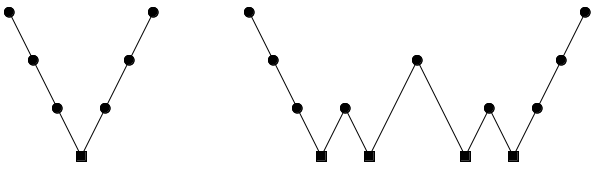
\includegraphics[width=\textwidth]{./Dsa/v_w_cycles}
\caption{$V-$ and $W-$cycle}
\end{figure}

For the theoretical discussion, the system matrix $\bs{A}$ is always assumed
to be symmetric and positive definite. The prolongation operators $P$ must
have full rank and the restriction $R$ and the coarse grid matrices $\bs{A}_H$
are defined by:
\begin{align}
&R=P^T\\
&\bs{A}_H = R\bs{A} P
\end{align}
Along with their corresponding norms $\|u\|_{\mc{H}^i} =
\sqrt{(u,u)_{\mc{H}^i}}$, $i\in \{0,1,2\}$, the scalar products:
\begin{align}
&(u,v)_{\mc{H}^0} = (D u,v)_2\\
&(u,v)_{\mc{H}^1} = (\bs{A} u, v)_2\\
&(u,v)_{\mc{H}^2} = (D^{-1} \bs{A} u, \bs{A}_v)_2
\end{align}
are needed. $D=diag(\bs{A})$ denotes the diagonal of $\bs{A}$. In some sense,
these are discrete counters part of the $H^{k}-$Sobolev (semi-)norms. In
algebraic error, an error $e$ is called smooth if is slow to converge with
respect to a smoother $S$. For example:
\begin{equation}
\|S e\|_{\mc{H}^1} \approx \|e\|_{\mc{H}^1}
\end{equation}
Depending on $\bs{A}$ an algebraically smooth error may well be highly
oscillation geometrically. For typical relaxation schemes like Gauss-Seidel,
the inequality:
\begin{equation}
\|S e\|_{\mc{H}^1}^2 \leq \|e\|_{\mc{H}^1}^2-\alpha \|e\|_{\mc{H}^2}^2
\label{gs_smooth_ineq}
\end{equation}
holds with $\alpha >0$ (e.g. $\alpha=1/4$). Therefore, an smooth error has to
satisfy $\|e\|_{\mc{H}^2} \ll \|e\|_{\mc{H}^1}$. Applying the Cauchy-Schwarz
inequality to $(\bs{A}e,e)_2 = \(\S^{-1/2}\bs{A}e, \bs{D}^{1/2} e\)_2$ shows:
\begin{equation}
\begin{split}
\|e\|_{\mc{H}^1}^2 &= \(D^{-1/2} \bs{A} e, D^{1/2} e\)_2\\
&\leq \|D^{-1/2} \bs{A} e\|_2 \|D^{1/2} e\|_2 = \| e \|_{\mc{H}^2}
\|e\|_{\mc{H}^0}
\end{split}
\end{equation}
Therefore, $\|e\|_{\mc{H}^2} \ll \|e\|_{\mc{H}^1}$ implies $\|e\|_{\mc{H}^1}
\ll \|e\|_{\mc{H}^0}$, or more explicitly:
\begin{equation}
\begin{split}
\(\bs{A} e,e\) &= \frac{1}{2} \sum_{i,j} -a_{i,j} (e_{i}-e_j)^2 + \frac{1}{2}
\sum_{i,j} a_{i,j} e_i^2 + \frac{1}{2} a_{i,j} e_j^2\\
&= \frac{1}{2} \sum_{i,j} -a_{i,j}(e_i-e_j)^2 + \sum_i \(\sum_j a_{i,j}\)
e_i^2 \ll \sum_i a_{i,i} e_i^2
\end{split}
\end{equation}
For the important case $\sum_{i\neq j} |a_{i,j}| \approx a_{i,i}$, this means
that, on the average for each $i$:
\begin{align}
&\frac{1}{2} \sum_{j\neq i} -a_{i,j} (e_i=e_j)^2 \ll a_{i,i} e_i^2\\
&\sum_{j\neq i} \frac{|a_{i,j}|}{a_{i,i}} \frac{(e_i-e_j)^2}{e_i^2} \ll 2
\end{align}
In other words, a smooth error generally varies slowly in the direction of
strong connections, i.e. from $e_i$ to $e_j$ if $\frac{|a_{i,j}|}{a_{i,i}}$ is
relatively large.

An important idea of the coarsening strategy is the strong connection.
\begin{definition}
A node $v_i \in V$ is strongly connected to a node $v_j \in V$ with respect to
$\bs{A}$ if:
\begin{equation}
-a_{i,j} \geq \theta \max_{m\neq i}(-a_{i,m})
\end{equation}
\end{definition}
\begin{definition}
$N_i^S$ denotes the set of all strongly connected neighbors of $v_i$:
\begin{equation}
N_i^S =\{ v_j \in N_i | -a_{i,j}\geq \theta \max_{m\neq i} (-a_{i,m})\}
\end{equation}
\end{definition}
\begin{definition}
The interpolatory nodes $C_i$ are the strong $C-$node neighbors:
\begin{equation}
C_i = N_i^S \cap C
\end{equation}
\end{definition}
\begin{definition}
The noninterpolatory nodes $D_i$ are split into strong$D_i^S$ and weak $D_i^W$
noninterpolatory nodes:
\begin{align}
& D_i = N_i \backslash C_i\\ 
& D_i^S = D_i \cap N_i^S\\
& D_i^W = D_i \backslash D_i^S
\end{align}
\end{definition}
Once again looking at:
\begin{equation}
a_{i,i} e_i \approx - \sum_{j} a_{i,j} e_j
\end{equation}
for a smooth vector $e$, we can expect that the interpolation of $e_j$,
$v_j\in D_i$:
\begin{equation}
e_j = \frac{\sum_{v_k \in C_i} |a_{j,k}| e_k}{\sum_{v_m \in C_i} |a_{j,m}|}
\end{equation}
is better for nodes $v_j$ which are strongly connected to the nodes in $C_i$.
If we add nodes to $C_i$, very likely the quality of the interpolation
increases. But on the other hand, the stencil sizes of the prolongation and
hence the stencil sizes of the coarse grid matrices and the numerical cost
grows. Therefore, the following criteria are taken as guidelines in order to
get good interpolations and a reasonable numerical complexity.
\begin{criterion}
For each node $v_i\in F$, each node $v_j\in N_i^S$ should either be in $C$, or
should be strongly connected to at least one node in $C_i$.
\label{crit_1}
\end{criterion}
\begin{criterion}
$C$ should be a maximal subset of all nodes with the property that no two
$C-$nodes are strongly connected to each other.
\label{crit_2}
\end{criterion}
Criterion (\ref{crit_1}) shall ensure that the interpolation is good enough
while criterion (\ref{crit_2}) enforces the coarsening algorithm to generate
coarse grids with significantly less nodes than the fine grid. Since it is not
always possible to satisfy strictly both criteria, criterion (\ref{crit_2}) is
only taken as guideline while criterion (\ref{crit_1}) must strictly be
satisfied.\\
The coarsening algorithm is divided into two steps. In the first step, a
relatively quick $C-$node choice is performed. $C-$nodes are distributed
uniformly over the grid attempting to enforce criterion (\ref{crit_2}). In the
second part the tentative $F-$nodes are tested to satisfy criterion
(\ref{crit_1}) and the interpolation weights are computed. Tentative $F-$nodes
not satisfying criterion (\ref{crit_1}) are labeled as $C-$nodes.
Sers de base of Ruge and Stuben

\section{Aggregation methods}
An iteration step of the aggregation algebraic multigrid methods is described
by algorithm (\ref{4_0_1}). The main difference to the interpolation methods
is the construction of the transfer operators and the coarse grids. In
interpolation methods, typically, each coarse grid degree of freedom has a
directly associated degree of freedom on the fine grid. Since aggregation
methods cluster on the fine grid unknowns to aggregates representing the
unknowns on the coarse grid, aggregation methods do not allow such a simple
identification of degrees of freedom on the coarse and the fine grid.

The standard one-dimensional model problem:
\begin{equation}
\bs{A}u=f,\ \bs{A}=
\begin{bmatrix}
-1 & 2 & -1
\end{bmatrix}
,\ \bs{A}\int\mathbb{R}^{n_h\times n_h}
\label{5_2_1}
\end{equation}
is considered. The application of the smoother $S$:
\begin{align}
& \bs{S} = \bs{I}-\frac{2}{3}\bs{D}^{-1}\bs{A}\\
& \bs{D} = diag(\bs{A})
\end{align}
to a vector $\phi=(0,\hdots,0,1,1,1,0,\hdots,0)^T$ yields the smoothed vector:
\begin{equation}
\bs{S}\phi =
\psi=\(0,\hdots,0\frac{1}{3},\frac{2}{3},1,\frac{2}{3},\frac{1}{3},0,\hdots,0\)^T
\end{equation}
Vectors of the form $\psi \in \mathbb{R}^{n_h}$ and $\phi \in
\mathbb{R}^{n_h}$ can be used as coarse grid basis vectors for a multigrid
algorithm. In that sense, the solution $u$ is approximated by a linear
combination of the coarse grid basis vectors:
\begin{align}
u \approx \sum_{i\leq n_H}\phi_i\cdot (u_H)_i &\Leftrightarrow
u\approx\bs{P}_{\phi} u_H,\ \bs{P}_{\phi} \int \mathbb{R}^{n_h\times n_H}\\
u \approx \sum_{i\leq n_H} \psi_i\cdot (u_H)_i &\Leftrightarrow
u\approx\bs{P}_{\psi} u_H,\ \bs{P}_{\psi}u_H,\ \bs{P}_{\psi}\in
\mathbb{R}^{n_h\times n_H}
\end{align}
where:
\begin{align}
&\bs{P}_{\phi} = (\phi_1,\hdots,\phi_{n_H})\\
&\bs{P}_{\psi} = (\psi_1,\hdots,\psi_{n_H})
\end{align}
Substituting $u$ in \cref{5_2_1} and multiplying both sides with
$\bs{R}_{\phi}\in \mathbb{R}^{n_H\times n_h}$ or $\bs{R}_{\psi} \in
\bs{R}^{n_H\in n_h}$ leads to the coarse grid systems:
\begin{align}
&\bs{R}_{\phi} \bs{A} \bs{P}_{\phi} u_H = \bs{R}_{\phi} f\\
&\bs{R}_{\psi} \bs{A} \bs{P}_{\psi} u_H = \bs{R}_{\psi} f
\end{align}
Note that, the number of degrees of freedom on the coarse grid $n_H$ generated
by $\bs{R}_{\phi}$, $\bs{P}_{\phi}$ or $\bs{R}_{\psi}$, $\bs{P}_{\psi}$ is
approximately $1/3$ of the number of fine grid unknowns ($n_H \approx 1/3
n_h$). The standard (1D) multigrid prolongation induced by the basis function
$(0,\hdots,0,1/2,1,1/2,0,\hdots,0)^T$ leads to a coarsening factor of about of
$1/2 (n_H\approx 1/2 n_h)$. Nevertheless, the prolongation $\bs{P}_{\psi}$ is
still a linear interpolation scheme. In two (or three) spatial dimensions, the
basis functions $\phi$ are constructed by clustering some unknowns to
so-called aggregates. Then, the basis function $\phi_i$ corresponding to the
aggregate $\mc{\bs{A}}_i$ is defined by:
\begin{equation}
\(\phi_i\)_j = \left\{
\begin{aligned}
&1 &\textrm{if }j\in \bs{\mc{A}}_i\\
&0 &\textrm{if }j\notin \bs{\mc{A}}_i
\end{aligned}
\right.
\end{equation}
Strongly coupled neighborhoods are aggregate.\\
Smoothed aggregation: 
\begin{enumerate}
\item aggregate the variables $\{\mc{\bs{A}}_i^l\}_{i=1}^{n_l+1}$
\item build a tentative prolongator $Y_{l+1}^l$
\item build the smoothed composite prolongator $\bs{P}_{0,l}$ defined by:
\begin{align}
&\bs{P}_{0,0} = \bs{I}\\
&\bs{P}_{0,l} = \bs{Z}_0 \bs{Y}_1^0\hdots \bs{Z}_{l-1} \bs{Y}_l^{l-1}
\end{align}
where $\bs{Z}_l$ denotes a prolongator smoother.
\end{enumerate}
The prolongation $\bs{P}_{l,l+1}$, the restriction $\bs{R}_{l+1,l}$ and the
coarse grid matrices $\bs{A}_{l+1}$ are defined by:
\begin{align}
&\bs{P}_{l,l+1} = \bs{Z}_l \bs{Y}_{l+1}^l\\
&\bs{R}_{l+1,l} = \(\bs{P}_{l,l+1}\)^T\\
&\bs{A}_{l+1} = \bs{R}_{l+1,l} \bs{A}_l \bs{P}_{l,l+1}
\end{align}
where $l=0,\hdots,l_{\max-1}$

\section{ML: Multilevel Preconditioning package}
\red{Pris de \cite{ml_guide}}\\
Some of the available coarsening schemes:
\begin{description}
\item [Uncoupled:] Attempt to construct aggregates of optimal size ($3^d$
nodes in $d$ dimensions). Each process works independently and aggregates
cannot span processes.
\item [MIS:] Uses maximal independent set techniques \cite{mis} to define
aggregates. Aggregates can span processes. May provide better quality
aggregates than \bf{Uncoupled}, but computationally more expensive because it
requires matrix-matrix product.
\end{description}
Some of the smoothers:
\begin{description}
\item [Jacobi]
\item [Symmetric Gauss-Seidel]
\end{description}
Some of the coarse solvers:
\begin{description}
\item [Jacobi]
\item [Symmetric Gauss-Seidel]
\item [Amesos-KLU:] Use \bf{KLU} through Amesos. Coarse grid problem is shipped to
proc 0, solved, and solution is broadcast.
\item [Amesos-UMFPACK:] Use \bf{UMFPACK} through Amesos. Coarse grid problem
is shipped to proc 0, solved, and solution is broadcast.
\item[Amesos-MUMPS:] Use double precision version of \bf{MUMPS} through
Amesos.
\end{description}
The MultiLevelPreconditioner class provides default values for five different
preconditioner types:
\begin{itemize}
\item Classical smoothed aggregation for symmetric positive definite or nearly
symmetric definite systems.
\item Classical smoothed aggregation-based 2-level domain decomposition.
\item 3-level algebraic domain decomposition,
\item Eddy current formulation of Maxwell's equations.
\item Energy-based minimizing smoothed aggregation suitable for highly
convective nonsymmetric fluid flow problems.
\end{itemize}
\begin{description}
\item [option name:] SA
\item [max levels:] 10
\item [prec type:] V-cycle
\item [aggregation type:] uncoupled-MIS
\item [aggregation damping factor:] 4/3
\item [eigen-analysis type:] cg
\item [eigen-analysis iterations:] 10
\item [smoother sweeps:] 2
\item [smoother damping factor:] 1.0
\item [smoother pre or post:] both
\item [smoother type:] symmetric Gauss-Seidel
\item [coarse type:] Amesos-KLU
\item [coase max size:] 128
\end{description}
\subsection{Smoothed Aggregation Options}
When performing smooth aggregation, the matrix graph is first coarsened
(actually vertices are aggregated together) and then a grid transfer operator
is constructed. A number of parameters can be altered to change the behavior
of these phases.\\
A graph of the matrix is usually constructed by associating a vertex with each
equation and adding an edge between two vertices $i$ and $j$ if there is a
nonzero in the $\(i,j\)^{th}$ or $(j,i)^{th}$ entry. It is this matrix graph
whose vertices are aggregated together that effectively determines the next
coarser mesh. Uncoupled aggregation and MIS aggregation schemes use fixed
ratio of coarsening between levels. Poorly done aggregation can adversely
affect the multigrid convergence and the time per iteration. In particular, if
the scheme coarsens too rapidly multigrid convergence may suffer. However, if
coarsening is too slow, the number of multigrid increases and the number of
nonzeros per row in the coarse grid discretization matrix may grow rapidly.
\subsection{Interpolation Options}
An interpolation operator is built using coarsening information, seed vectors,
and a damping factor. Coarsening or aggregation information or first used to
create a tentative interpolation operator. This process takes a seed vector or
seeds vectors and builds a grid transfer operator. It is important to
understand that only a few seed vectors are needed and that these seed vectors
should correspond to components that are difficult to smooth. The tentative
interpolation that results from these vectors will interpolate the seed
vectors perfectly. It does this by ensuring that all seed vectors are in the
range of the interpolation operator. This means that each seed vector can be
recovered by interpolating the appropriate coarse grid vector. The general
idea of multigrid methods is that errors not eliminated by the smoother must
be removed by the coarse grid solution process. If the error after several
smoothing iterations was known, it would be possible to pick this error vector
as the seed vector. However, since this is not the case, we look at vectors
associated with small eigenvalues (or singular values in the nonsymmetric
case) of the discretization operator. Errors in the direction of these
eigenvectors are typically difficult to smooth as they appear much smaller in
the residual ($r=\bs{A}e$ where $r$ is the residual, $\bs{A}$ is the
discretization matrix, and $e$ is the error). For most scalar PDEs, a single
seed vector is sufficient and so we seek some approximation to the eigenvector
associated with the lowest eigenvalue. It is well known that a scalar Poisson
operator with Neumann boundary conditions is singular and that the null space
is the constant vector. Thus, when applying smoothed aggregation to Poisson
operators, it is quite natural to choose the constant vector as the seed
vector. In many cases, this constant vector is a good choice as all spatial
derivatives within the operator are zero and so it is often associated with
small singular values. Within ML the default is to choose the number of seed
vectors to be equal to the number of DOFs at each node. Each vector
corresponds to a constant vector for that DOF component. Specifically, if we
have a PDE system with two DOFs per node. Then one seed vector is one ate the
first DOF and zero at the other DOF throughout the graph. The second seed
vector is zero at the first DOF and one at the other DOF throughout the graph.
In some cases, information is known as to what components will be difficult
for the smoother or what null space is associated with an operator. Once the
tentative prolongator is created, it is smoothed via a damped Jacobi
iteration. The reasons for this smoothing are related to the theory where the
interpolation basis functions must have a certain degree of smoothness.
However, the smoothing stage can be omitted by setting the damping to zero.
Though theoretically poorer, unsmoothed aggregation can have considerably less
set up time and less cost per iteration than smoothed aggregation. When
smoothing, ML has a few ways to determine the Jacobi damping parameter and
each require some estimate of the spectral radius of the discretization
operator. The current default is to use a few iterations of the power method
(subspace size of two) to estimate this value. However if the matrix is
symmetric conjugate-gradient method should be used.

\section{Tire de \cite{mis} MIS = Maximally Independent Sets}
Multilevel methods offer the best promise to balance fast convergence and
parallel efficiency in the numerical solution of elliptic partial differential
equations. Multigrid methods are scalable and relatively suitable for parallel
implementation. The idea of multigrid is to capture arroses spanning a range of
spaces via several levels of fineness. By traversing the levels, optimal
convergence rates are frequently observed (independent of the number of mesh
points) with overall solution times that are much faster than other methods.

The $\bs{P}_k$ (interpolation operators that transfer solutions from coarse
grids to finer grids) are the key ingredients that must be determined
automatically within an algebraic multigrid method. The smooth aggregation
$\bs{P}_k$ are determined in two steps: coarsening and grid transfer
construction. The first step is to take each grid point and assign it to an
aggregate. The second step consists of first forming a tentative prolongator
matrix $\bs{\tilde{P}}_k$ and then applying a prolongator smoother
$\bs{\tilde{S}}_k$ to it giving rise to $\bs{P}_k=\bs{\tilde{S}}
\bs{\tilde{P}}_k$. The tentative prolongator matrix $\bs{\tilde{P}}_k$ is
constructed such that each row corresponds to an aggregate. The entries of
$\bs{\tilde{P}}_k$ are as follows (for specific applications such as
elasticity problems, more complicated tentative prolongators can be derived
based on rigid body motions):
\begin{equation}
\bs{\tilde{P}}_k(i,j) = \left\{
\begin{aligned}
&1 &\textrm{if $i^{th}$ point is contained in $j^{th}$ aggregate}\\
&0 &\textrm{otherwise}
\end{aligned}
\right.
\end{equation}
The tentative prolongator can be viewed as a simple grid transfer operator
corresponding to piecewise constant interpolation. While $\bs{\tilde{P}}_k$
can be used for $\bs{P}_k$, a more robust method is realized by smoothing the
piecewise constant basis functions. For example, applying a damped Jacobi
smoother yields:
\begin{equation}
\bs{P}_k = \(\bs{I}-\omega \bs{D}_k^{-1} \bs{A}_k\) \bs{\tilde{P}}_k
\label{smooth_prolongator}
\end{equation}
If $\omega$ and the aggregates are properly chosen, \cref{smooth_prolongator}
leads to linear interpolation when applied to an one-dimensional Poisson
problem. In general, \cref{smooth_prolongator} does not correspond to linear
interpolation but yields better interpolation properties than piecewise
constant interpolation. We now return to the first step of determining the
$\bs{P}_k$. The generation of tentative prolongator requires that aggregates
be defined. For isotropic problems using the above damped Jacobi smoother, the
goal is to have fairly uniform shaped aggregate regions with a diameter of
length three. Small aggregates (diameter less than three) lead to high
iteration costs. This is because the number of unknowns on the next finest
grid is equal to the number of aggregates and because the number of nonzeros
per row in the coarse grid discrete operator depends on the distance between
non-neighboring aggregates. However, aggregates that are too large lead to
grid transfer operators that look more like piecewise constant interpolation
and give poorer convergences rates. The basic aggregation procedure (like the
one used in Uncoupled) is given below (graph is made only of the strong
connection):
\begin{description}
\item [Phase 1:] repeat until all unaggregated points are adjacent to an
aggregate:
\begin{enumerate}
\item pick root point not adjacent to any existing aggregate
\item define new aggregate as root point plus all its neighbors
\end{enumerate}
\item [Phase 2:] sweep unaggregated points into existing aggregates or use
them to form new aggregates
\end{description} 


\red{Pris de \cite{smooth_agg_conv}}\\
In our AMG method, we build the prolongation operators by first constructing
a tentative prolongation using an approach and the knowledge of zero energy
modes of the equation, then smoothing its output by a carefully selected
iteration. Matrix data and zero energy modes are the input of other widely
used iterative methods. The use of zero energy modes has become a recognized
way to capture the essential information needed to build an efficient
iterative method. We are interested in solving the system of linear algebraic
equations:
\begin{equation}
\bs{A}x=b
\end{equation}
where $\bs{A}$ is a symmetric positive definite matrix. The smoothed
aggregation multigrid can be viewed as a standard variational multigrid method
with prolongators of the form $\bs{S}_l \bs{P}_{l+1}^l$, where $\bs{P}_{l+1}^l
: \mathbb{R}^{n_l+1}\rightarrow \mathbb{R}^{n_l}, n_1 = ord(\bs{A}) >n_2>
\hdots > n_L$ is the full-rank tentative prolongator and $\bs{S}_l :
\mathbb{R}^{n_l}\rightarrow \mathbb{R}^{n_l}$ is a prolongator smoother
derived from the matrix $\bs{A}_l$. The hierarchy of coarse level matrices is
defined by:
\begin{align}
&\bs{A}_{l+1} = \(\bs{S}_l \bs{P}_{l+1}^l \)^T \bs{A}_l \bs{S}_l
\bs{P}_{l+1}^l\\
&\bs{A}_1 = \bs{A}
\end{align}
Although we will carry out some convergence estimates for general prolongators
smoothers $\bs{S}_l:\mathbb{R}^{n_l}\rightarrow \mathbb{R}^{n_l}$, the form of
$\bs{S}_l$, we use is:
\begin{equation}
\bs{S}_l = \bs{I} - \frac{4}{3 \bar{\lambda}_l^M}\bs{M}_l^{-1} \bs{A}_l
\end{equation}
Here, $\bar{\lambda}_l^M > \rho\(\bs{M}_l^{-1}\bs{A}_l\)$, $\rho$ denotes the
spectral radius, and:
\begin{align}
&\bs{M}_l =\(\bs{P}_l^1\)^T \bs{P}_l^1\\
&\bs{P}_l^1=\bs{P}_2^1\hdots \bs{P}_l^{l-1}\\
&\bs{P}_1^1 = \bs{I}
\end{align}
The mapping $\bs{P}_l^1:\mathbb{R}^{n_l} \rightarrow \mathbb{R}^{n_1}$ is
called composite tentative prolongator. The parameter 4/3 on level $l$
minimizes the value of $\rho\(\bs{M}_{l+1}^{-1} \bs{A}_{l+1}\)$.


\red{Pris de \cite{amg_unstruc}}\\
The first approach to such matrix based multigrid was the AMG code of Ruge et
al. This code introduced the concept of strongly coupled nodes and attempted
to find a coarsening from the condition that interpolation should prefer to
proceed along strong couplings. The associated interpolations were based on
the condition of flux preservation exploiting the condition that the kernel of
the matrix consists of constant functions (aside from boundary conditions).
Since constant functions can be expressed easily without knowing much about
the problem, the resulting solver could be formulated in terms of the matrix
only. We use the concept of strong connections to select our aggregates of
nodes, which play a role similar to Ruge's coarse points. The theory for AMG
was based on two-level estimates which do not give convergence bounds
independent of the number of levels. The deterioration of convergence was
indeed observed, and to defeat this, relatively many coarse points had to be
selected, resulting in less attractive computational complexity. Our approach
is based on the concept of smoothed aggregation. First the set of nodes is
decomposed into small mutually disjoint subsets. A tentative piecewise
constant interpolation (in the discrete sense) is then defined using this
decomposition. The final interpolation operator is obtained by smoothing the
result of such piecewise constant interpolation. The coarse level operatores
are then defined variationally. The resulting method converges very fat for a
wide range of problems including those with strongly anisotropic and
discontinuous coefficients. In addition, the new method has remarkably low
computational complexity since our typical coarsening ratio is bout three in
each dimension.

\section{AGMG \cite{agmg_guide}}
AGMG is a fortran library which is written in fortran 90 and use the MUMPS
library for the direct solver.

\red{pris de \cite{k_cycle}}\\
Multigrid methods were initially designed as stand-alone solvers, and they are
quite successful as such in many applications, for which one may refer to the
so-called ``textbook multigrid efficiency'' (meaning that the solutions to the
governing system of equations are attained in a computational work which is a
small (less than 10) multiple of the operation count in the discretized system
of equations (residual evaluations)). However MG methods, especially their
algebraic variants are nowadays used in applications for which such efficiency
is yet to be achieved. One common way to somewhat improve their robustness is
to use them as preconditioners in a Krylov subspace iterative method, for
instance, in the conjugate gradient (CG) method if the system matrix is
symmetric positive definite (SPD). Now, this still may not be sufficient to
provide fast convergence if the two-grid convergence factor is too large to
allow convergence properties independent of the number of levels with $V-$ or
$W-$cycles. Moreover, in real-life problems, it is often impossible to predict
if such a situation will occur of not, and the type of cycle that would be
optimal. This motivates us to consider Krylov-based MG-cycles (or K-cycle, for
short). With these cycles, the MG method is still based on the recursive use
of a two-grid method, but the needed coarse-grid solve is defined by a few
steps of a Krylov subspace iterative method with the already defined (by
recursion) MG method on the previous (coarser) level as preconditioner. If
$\mu$ inner iterations are performed at each level, we have more specifically
a $K_{\mu}-$cycle preconditioner. Such an idea is not new; it has been used,
also in a multilevel setting, for the co-called AMLI methods. The latter can
be viewed as stabilized versions of the hierarchical basis methods. The
stabilization comes from more than one recursive calls of the preconditioner
defined (by recursion) at a given level. Observe that the MG preconditioner
defined in this way becomes a nonlinear operator and thus the analysis of such
techniques is not as straightforward.
\begin{algorithm}
MG as preconditioner at level $k$ $(k\geq 1)$\\
Input: $r_k$; output: $z_k$:
\begin{enumerate}
\item Relax $\nu_k$ times using smoother $\bs{M}_k$: $v_k =
\(\bs{I}-\(\bs{I}-\bs{M}_k^{-1}\bs{A}_k\)^{\nu_k}\)\bs{A}_k^{-1}r_k$
\item Compute new residual: $\tilde{r}_{k-1} = r_k - \bs{A}_k v_k$
\item Restrict residual: $r_{k-1} = \bs{P}_k^T \tilde{r}_k$
\item Compute an (approximate) solution $y_{k-1}$ to $\bs{A}_{k-1} x_{k-1} =
r_{k-1}$
\item Interpolate coarse-grid correction: $y_k=\bs{P}_k y_{k-1}$
\item Compute new residual: $\bar{r}_k=\tilde{r}_k - \bs{A}_ky_k$
\item Relax $\nu_k$ times using smoother $\bs{M}_k^T$:
$w_k=\(\bs{I}-(\bs{I}-\bs{M}_k^{-T}\bs{A}_k)^{\nu_k}\)\bs{A}_k^{1})\bar{r}_k$
\item $z_k = v_k+y_k+w_k$
\end{enumerate}
\label{k_cycle_algo}
\end{algorithm}
If an exact solution is computed at step 4, the algorithm \ref{k_cycle_algo} 
computes the action $z_k-\bs{B}_k^{-1} r_k$ of the two-grid preconditioner 
$\bs{B}_k$ satisfying the relation:
\begin{equation}
\bs{I}-\bs{B}_k^{-1} \bs{A}_k = (\bs{I}-\bs{M}_k^{-T} \bs{A}_k)^{\nu_k}
(\bs{I}-\bs{P}_k \bs{A}_{k-1}^{-1} \bs{P}_k^T \bs{A}_k) (\bs{I}-\bs{M}_k^{-1}
\bs{A}_k)^{\nu_k}
\end{equation}
Note that our general assumptions imply that $\bs{B}_k$ is SPD. Now, in
practice, an exact solution is typically computed ate step 4 only for $k=1$
(that is, only matrix $\bs{A}_0$ on the coarsest grid is inverted exactly).
For $k>1$, the MG preconditioner at level $k$ computes $y_{k-1}$ approximately
using the MG preconditioner at level $k-1$. The way this is done defines the
so-called cycling strategy. Standard cycles are $V-$ and $W-$cycles;
$V-$cycles use only one action of the preconditioner on the coarser level,
whereas $W-$cycles preform two stationary iterations. Here, we define the
$K_{\mu}-$cycle MG preconditioner as the preconditioner implemented by
algorithm \ref{k_cycle_algo} when the coarse-grid system at step 4 is solved
by $\mu$ iterations of a Krylov subspace iterative method using the
$K_{\mu}$-cycle preconditioner on the coarser level, until level $k=1$ where
the two-grid preconditioner $B_1$ is used. At level $k$, we denote this
preconditioner $\mc{K}_{\mu}^{(k)}$. In general, this is a nonlinear operator,
this for the vector computed by algorithm \ref{k_cycle_algo} we write $z_k =
\mc{K}_{\mu}^{(k)}[r_k]$. In some cases, it is better to allow inner
iterations only at levels of given multiplicity $k_0>1$, that is, at levels
$l-k_0,l-2k_0,\hdots$. At other levels, inner iterations are skipped and a
simple $V-$cycle formulation is used. The $K_{\mu}^{(k,k_0,l)}-$cycle MG
preconditioner $\mc{K}_{\mu}^{(k,k_0,l)}[\cdot]$ is then defined as follows.
For $k=1$, this is as above the two-grid preconditioner:
$\mc{K}_{\mu}^{(1,k_0,l)}\[\cdot\] = \bs{B}_1^{-1}$. For
$k=2,3,\hdots,\mc{K}_{\mu}^{(k,k_0,l)}$ is recursively defined as the
preconditioner implemented by algorithm \ref{k_cycle_algo} at level $k$ with,
at step 4:
\begin{itemize}
\item If mod $(l-(k-1),k_0)=0$, then $y_{k-1}$ is computed by solving
$\bs{A}_{k-1} x_{k-1} = r_{k-1}$ with $\mu$ iterations of a Krylov subspace
iterative method using preconditioner $\mc{K}_{\mu}^{(k-1,k_0,l)}$.
\item Otherwise, we let $y_{k-1} = \mc{K}_{\mu}^{(k-1,k_0,l)}\[\cdot\]$.
\end{itemize}
Here, we consider the flexible CG method \cite{fcg,fcg_2,fcg_3,fcg_4}. In the
context of $K-$cycle MG preconditioner, this algorithm will be invoked at step
4 of algorithm \ref{k_cycle_algo} with $\bs{A}=\bs{A}_{k-1}$, $b=r_{k-1}$,
$\mc{B}=\mc{K}_{\mu}^{(k-1,k_0,l)}$, and the computed solution $x_{i+1}$ at
step 3 of the final iteration will give the needed $y_{k-1}$. This algorithm
will then also be helpful as outer solver for the main system, since the
top-level preconditioner $\mc{K}_{\mu}^{(l,k_0,l)}$ is also nonlinear. For
difficult problems, for which $V-$cycle is slow, $K-$cycle MG can be much more
effective than $W-$cycle MG. $K-$cycle MG appears more robust than $W-$cycle
MG. It can exhibit convergence properties independent of the number of levels
even when the condition number for the underlying two-grid method is
relatively large. Using $K-$cycles may thus enhance the robustness of a MG
method, in particular that of AMG schemes for real-life problems. This
enhances robustness is obtained nearly for free since the $K-$cycle has
roughly the same computational complexity as the $W-$cycle. Finally, sometimes
the number of unknowns does not decrease sufficiently fast from one level to
the next to allow inner iterations at each level as foreseen with standard
$K-$ or $W-$cycles. To cope with such cases, we introduces a variant of
$K-$cycle MG that allows inner iterations only at levels of given multiplicity
$k_0>1$, whereas a $V-$cycle formulation is used at other levels.

\red{Pris de \cite{agmg2}}\\
We consider more particularly aggregation-based multigrid schemes, in which
the hierarchy of coarse systems is obtained from a mere aggregation of the
unknowns. This approach is obtained from a mere aggregation of the unknowns.
This approach is sometimes referred to as ``plain'' or ``unsmoothed''
aggregation, to distinguish it from ``smoothed aggregation AMG''. It has some
appealing features such as cheap setup stage and memory requirements. However,
it is somehow nonstandard because it does not mimic any well-established
geometric multigrid method. We analyze the basic two-grid method for a class
of matrices which include symmetric $M$-matrices with nonnegative row sum
(that is, weakly diagonally dominant matrices with non positive off diagonal
entries). We show that the convergence rate can be bounded assessing for each
aggregate a local quantity which in some sense measure its quality, the bound
being determined by the worst aggregate's quality. Moreover, this bound seems
able to accurately predict the actual convergence, at least when applied to
PDEs discretized on regular grids with regular (geometric based) aggregation
patterns. However, these results suffer from two important limitations.
Firstly, they are only for a model two-grid scheme. In practice, the method
has to be recursively used in a multigrid cycle, and no guarantee is given
that the convergence rate will then remain optimal; i.e., will not deteriorate
with the number of levels. Next, the analysis can in principle be applied to
any ``algebraic'' aggregation algorithm that automatically builds aggregates
inspecting connections in the system matrix. However, as a general rule, such
algorithms tend to always produce a limited number of badly shaped aggregates,
and, since the bound is determined by the worst aggregate's quality, even a
few of these can significantly impact the resulting bound. The latter is also
difficult to predict in case of PDEs discretized on unstructured grids. Hence,
although we have proper tools to assess aggregation-based two-grid methods,
what can actually be proved for a truly algebraic method remains unclear. Here
we overcome these limitations mainly by introducing a new aggregation
algorithm based on the explicit control of aggregate's quality. It tens to
optimize the latter while imposing some minimal requirements; i.e., the
algorithm has as main input parameter the upper bound on the two-grid
condition number that is required to hold. Of course, such an approach
potentially induces an increase of the algorithmic complexity. In the
multigrid context, mastering the complexity means ensuring that the cost of
each iteration step does not grow more than linearly with the number of the
unknowns. Taking into account that the two-grid method has to be used
recursively, this further means ensuring that the number of unknowns decreases
sufficiently fast from one level to the next. With aggregation-based methods,
the factor by which the number of unknowns is decreased is actually the mean
aggregates' size (i.e., the mean number of unknowns inside an aggregate).
Whereas with heuristic aggregation algorithms it is relatively easy to control
this mean aggregates' size, the present approach introduces more uncertainty:
one may form aggregates of a given target size, but there is no a priori
guarantee that they will satisfy the quality criterion that allows to control
the condition number. All in all, there are two advantages in controlling
explicitly the convergence rate (or the condition number) instead of the
complexity. Firstly, in a typical situation, a ``complexity oriented''
algorithm will form a few badly shaped aggregates. As already mentioned, this
may have a dramatic impact on the convergence analysis. If there are only a
few such bad aggregates, their influence on the actual convergence may or not
be significant, in general we just don't know. An algorithm that explicitly
controls the condition number will refuse to form these bad aggregates and
stay instead with a few aggregates of smaller size or even some unaggregated
nodes. Compared with the previous situation, here we know that if there is
only a small amount of such aggregates, then the impact on the efficiency of
the method will be minor, since it would only affect the mean aggregates' size
in a unessential way. A second advantage of the approach is that it fits well
with the use of the so-called AMLI-cycle. With this cycle, the iterative
solution of the coarse system at each level is accelerated with a
semi-iterative method based on Chebyshev polynomials. As main advantage, this
cycle allows to build optimal multigrid schemes using only two-grid analysis.
More precisely, this will be possible if there is an known upper bound
$\bar{\kappa}_{TG}$ on the condition number of the two-grid method at every
level and an integer $\gamma$ (related to the degree of Chebyshev polynomials)
such that:
\begin{equation}
\sqrt{\bar{\kappa}_{TG}} < \gamma < \tau
\end{equation}
where $\tau$ stands for the mean factor by which the matrix size is reduced
from one level to the next. Both inequalities should be interpreted in a
restrictive way: for an efficient method, $\sqrt{\bar{\kappa}_{TG}}$ should be
substantially away from $\gamma$ and this latter itself substantially away
from $\tau$. The left inequality guarantees that the condition number remains
bounded even for infinitely many levels, and the right one ensures an optimal
computational complexity. That said, the left inequality is the most difficult
to deal with because, recall, it has to be checked by an upper bound on the
two-grid condition number, which has to hold at every level of the hierarchy,
and, further, to be known explicitly because it enters the definition of the
parameters of the AMLI-cycle. Therefore, by introducing a new approach the use
of the AMLI-cycle, which is here seemingly for the first time combined with a
truly algebraic multigrid. The system matrix $\bs{A}$ to be a symmetric
$M$-matrix with nonnegative row sum. We first introduce some (related to our
two-grid setting). We consider symmetric two-grid schemes, using symmetric
positive two-grid schemes, using symmetric positive definite smoother $\bs{M}$
with one pre- and one post-smoothing step. We also assume that the coarse grid
matrix is of Galerkin type; that is, given $n \times n_c$ prolongation matrix
$\bs{P}$, the coarse grid matrix is $\bs{A}_c = \bs{P}^T \bs{A} \bs{P}$. The
corresponding iteration matrix is then:
\begin{equation}
\bs{T} = (\bs{I}-\bs{M}^{-1} \bs{A}) (\bs{I}-\bs{P}\bs{A}_c^{-1}\bs{P}^T
\bs{A}) (\bs{I}-\bs{M}^{-1} \bs{A})
\end{equation}
which also implicitly defines the two-grid preconditioner $\bs{B}_{TG}$ via
the relation:
\begin{equation}
\bs{I}-\bs{B}_{TG}^{-1}\bs{A}=\bs{T}
\end{equation}
Equivalently, one has:
\begin{equation}
\bs{B}_{TG}^{-1} = \bs{M}^{-1} (2\bs{M} - \bs{A}) \bs{M}^{-1} +
(\bs{I}-\bs{M}^{-1} \bs{A}) \bs{P} \bs{A}_c^{-1} \bs{P}^T
(\bs{I}-\bs{A}\bs{M}^{-1})
\end{equation}
Now, with the coarsening by aggregation, the prolongation is obtained from the
agglomeration of the unknowns into $n_c$ nonempty disjoint sets $G_k,
k=1,\hdots,n_c$, called aggregates. To each aggregate $G_k$ is associated one
unknown at the next coarse level in the hierarchy. Besides, some unknowns can
be also kept outside the coarsening process, and the corresponding (possible
empty) set is noted $G_0$; that is, $G_0$ gathers the unknowns that are not
associated to any coarse unknown. As a result, $G_0$ together with
$G_k,k=1,\hdots,n_c$, defines a partitioning of the index set $[1,n]$ which
uniquely determines the prolongation $\bs{P}$: for $i=1,\hdots,n$ and
$j=1,\hdots,n_c$:
\begin{equation}
\bs{P}_{ij} = \left\{
\begin{aligned}
&1 & \textrm{if }i\in G_j\\
&0 & \textrm{otherwise}
\end{aligned}
\right.
\end{equation}
Hence a row of $\bs{P}$ is zero if and only if the corresponding unknown is in
$G_0$, whereas the other rows have exactly one nonzero entry. Note that that
the entries in the coarse grid matrix $\bs{A}_c=\bs{P}^T\bs{A}\bs{P}$ can be
obtained from a simple summation process:
\begin{equation}
\bs{A}_{c,kl} = \sum_{i\in G_k} \sum_{j\in G_l} a_{ij} \ \ k,l=1,\hdots,n_c
\end{equation}
It follows from this relation that if $\bs{A}$ is an M-matrix with nonnegative
row sum, then $\bs{A}_c$ inherits form these properties.

The aggregation scheme considered in this work is based on a few passes of a
pairwise matching algorithm, which amounts to group into pairs. The qualities
$\mu(G)$ is a inferior bound of the two-grid condition numbers.

A naive approach when trying to build high quality aggrgates of desired size
would be to explore the matrix graph while testing all suitable aggregates.
This is a costly strategy, because of the often important number of
possibilities and the need to compute the quality estimate for each of them.
An alternative would be to guess a few potentially interesting aggregates of
targeted size or above and choose the most appropiate. Here, we follow this
latter idea by considering an aggregation procedure based on a few passes of a
pairwise algorithm, which attempts to group unknowns into pairs. This approach
is inspires by the double pairwise aggregation algorithm in \cite{agmg},
which, although based on heuristic arguments, was found able to build sensible
aggregates in an inexpensive way. Further motivation comes from the fact that,
when there are only two unknowns in $G$, the quality $\mu(G)$ reduces to an
easy-to-compute function involving only the off-diagonal entry connecting
these two unknowns, their respective diagonal entries, and the sum of all
off-diagonal elements in the corresponding rows. Therefore, pre-computing the
latter, it is inexpensive to find the best pair that contains a given unknown.
On the other hand, we observe that, whereas assessing $\mu(G)$ for large $|G|$
may become costly, it remains relatively cheap to check that $\mu(G)\leq
\bar{\kappa}_{TG}$ for a given threshold. Indeed, this condition holds if and
only if:
\begin{equation}
\bar{\kappa}_{TG} \bs{A}_G - \bs{M}_G (\bs{I} -
\bs{1}_G(\bs{1}_G^T\bs{M}_G\bs{1}_G)^{-1} \bs{1}_G^T \bs{M}_G)
\end{equation}
is nonnegative definite, which is true if and only if the Cholesky
factorization of this matrix exists (i.e., no pivot is negative). Hence, the
requirement (ii) of theorem 2.1 can be checked in only $\mc{O}(|G|^3)$
operations. This is taken into account in our aggregation in the aggregation
procedure, which allows to ensure that all aggregates satisfy the needed
quality requirement, and hence that the relation (2.8) holds, while avoiding
an explicit computation of $\mu(G)$ for any subset $G$ with more than two
unknowns. Now the initial pairwise aggregation as applied during the first
pass is presented in algorithm \ref{4_1}. It is largely inspired by theorem
2.1. One first forms the set $G_0$ of unknowns that can be kept outside the
aggregation by checking wether the condition (2.6) holds. Next one picks up an
unknown at a time and searches, among its still unassigned neighbors, the one
yielding the pair with the best quality. Then, it is checked wether or not
this quality satisfies the acceptance criterion; if not, the unknown initially
picked up remains unassociated in the coarse grid. To obtain large aggregates,
we compute the auxiliary coarse grid matrix $\tilde{A} = \tilde{a}_{ij}$
corresponding to this initial pairwise aggregation. Then, we apply essentially
the same algorithmm to this matrix to form pairs or pairs; or, in subsequent
applications, pairs of aggregates from the previous pass. However, some care
is needed beacute both conditions (2.6) and (2.7) are to be checked in the
initial matrix. In particular, the set $G_0$ has to remain the one initially
defined during the first pass. Furthermore, the estimate
$\tilde{\mu}(\{i,j\})$ used ti assess the quality of the pair $\{i,j\}$ has to
be adapted so as to correctly reflect the quality of the corresponding
aggregate $\mu(G_i \cup G_j)$ in the original matrix. This is obtained by
using the same formula as in algorithm \ref{4_1} but changing slightly the
definition of $\tilde{s}_i$. This change is needed to ensure that if
$\tilde{\mu}\(\{i,j\}\)$ is a lower bound on $\mu(G_i\cup G_j)$. It means that
if $\tilde{\mu}(\{i,j\})$ is above the threshold, the pair should anyway be
rejected because $\mu(G_i\cup G_j)$ cannot be smaller than
$\bar{\kappa}_{TG}$. It also means that $\tilde{\mu}(\{i,j\}) \leq
\bar{\kappa}_{TG}$ can only be a prelimnary acceptance criterion, which has to
be supplemented by an explicit check that $\mu(G_i\cup G_j)\leq
\bar{\kappa}_{TG}$; however, as indicated above, this can be done by
factorizing a $|G_i \cup G_j|\times |G_i \cup G_j|$ matrix. These
considerations lead to algorithm \ref{4_2}. Eventually, we make explicit in
algorithm \ref{4_3} how these pariwise aggregation procedures are put
together. An uncommon feature is that one can perform an arbitrary number of
passes of pairwise aggregation wihout degrading the upper bound on the
condition number number. In practice, the process is stopped either if the
specified maximal number of passes has been reached or once the coarsening
factor is above a given target.
\begin{algorithm}
Initial pairwise aggregation:\\
\begin{description}
\item [input:] $n \times n$ matrix $\bs{A} = (a_{ij})$ and thresold
$\bar{\kappa}_{TG}$
\item [output:] $n_c$ and sets $G_0,\hdots,G_{n_c}$
\end{description}
\begin{description}
\item [Initialize:] 
\begin{align}
&G_0 = \left\{ i \big| a_{ii} \geq
\frac{\bar{\kappa}_{TG}+1}{\bar{\kappa}_{TG}-1} \(\sum_{\substack{k=1\\ k\neq
i}}|a_{ik}|\)\right\} \nonumber \\
& U \leftarrow [1,n]\backslash G_0 \nonumber \\
&n_c \leftarrow 0 \nonumber \\
&s_i \leftarrow - \sum_{j\neq i} a_{ij} \ \forall i \in U \nonumber
\end{align}
\item [Iterate:] while $U \neq \emptyset$ do:
\begin{itemize}
\item Select $i\in U$
\item Find $j\in U\backslash \{i\}$ such that $a_{ij} \neq 0$ and $\mu
\(\{i,j\}\) = \frac{-a_{ij} + \(\frac{1}{a_{ii}+s_i+2 a_{ij}}+\frac{1}{a_jj+s_j
+2 a_{ij}}\)^{-1}}{-a_{ij} + \(\frac{1}{a_{ii}-s_i} +
\frac{1}{a_{jj}-s_j}\)^{1}}$ is minimal
\item $n_c \leftarrow n_c+1$
\item if $(\mu(\{i,j\}) \leq \bar{\kappa}_{TG})$ $G_{n_c}=\{i,j\};$
$U\leftarrow U\backslash \{i,j\}$
\item else $G_{n_c} = \{i\}$; $U\leftarrow U\backslash \{i\}$
\end{itemize}
\end{description}
\label{4_1}
\end{algorithm}

\begin{algorithm}
Further pairwise aggregation\\
\begin{description}
\item [input:] \hbox{}
\begin{itemize}
\item[] $n\times n$ matrix $\bs{A}=(a_{ij})$
\item[] threshold $\bar{\kappa}_{TG}$
\item[] tentative $\tilde{n}_c$ and sets $\tilde{G}_k, k=1,\hdots, n_c$
\item[] corresponding $\tilde{n}_c \times \tilde{n}_c$ matrix $\bs{\tilde{A}}
= (\tilde{a}_{ij})$
\end{itemize}
\item [output:] $n_c$ and sets $G_1,\hdots,G_{n_c}$
\end{description}
\begin{description}
\item [Initialize:] \hbox{}
\begin{align}
& U \leftarrow [1,\tilde{n}_c] \nonumber \\
& n_c \leftarrow 0 \nonumber \\
&\tilde{s}_i \leftarrow - \sum_{k\in G_i}  \sum_{j \in G_i} a_{kj} \ \forall i
\in U \nonumber \\
\end{align}
\item [Iterate:] while $U \neq \emptyset$ do:
\begin{itemize}
\item Select $i \in U$
\item Set $T=\{ j \| \tilde{a}_{ij} \neq 0 \textrm{ and } \tilde{\mu}(\{i,j\})
\leq \bar{\kappa}_{TG}\}$, where $\tilde{\mu}(\{i,j\}) =
\frac{-a\tilde{a}_{ij} +
\(\frac{1}{\tilde{a}_{ii}+\tilde{s}_i+2\tilde{a}_{ij}} +
\frac{1}{\tilde{a}_{jj}+\tilde{s}_j + 2
\tilde{a}_{ij}}\)^{-1}}{-\tilde{a}_{ij}+\(\frac{1}{\tilde{a}_{ii}-\tilde{s}_i}+
\frac{1}{\tilde{a}_{jj}-\tilde{s}_j}\)^{-1}}$
\item $n_c \leftarrow n_c+1$
\item if $(T\neq \emptyset)$:
\begin{itemize}
\item Select $j\in T$ with minimal $\tilde{\mu}\(\{i,j\}\)$
\item if $\(\mu\(\tilde{G}_i \cup \tilde{G}_j\) \leq \bar{\kappa}_{TG}\)$
$G_{n_c} = \tilde{G}_i \cup \tilde{G}_j$; $U \leftarrow U \backslash \{i,j\}$
\item else $T\leftarrow T\backslash \{i\}$; goto if $(T\neq \emptyset)$
\end{itemize}
\item else $G_{n_c} = \tilde{G}_i$; $U \leftarrow U\backslash \{i\}$
\end{itemize}
\end{description}
\label{4_2}
\end{algorithm}

\begin{algorithm}
Multiple pariwise aggregation\\
\begin{description}
\item [input:] \hbox{}
\begin{itemize}
\item[] $n\times n$ matrix $\bs{A}$
\item[] threshold $\bar{\kappa}_{TG}$
\item[] maximal number of passes $n_{pass}$
\item[] target coarsening factor $\tau$
\end{itemize}
\item [output:] \hbox{}
\begin{itemize}
\item $n_c$ ans sets $G_0,\hdots,G_{n_c}$
\item corresponding aggregation matrix $\bs{A}_c$
\end{itemize}
\end{description}
\begin{description}
\item[First pass:] \hbox{}
\begin{itemize}
\item[] Apply Initial pairwise aggregation algorithm  to matrix $\bs{A}$ with
threshold $\bar{\kappa}_{TG}$; Output: $n_c^{(1)}, G_0$ and
$G_1^{(1)},\hdots,G_{n_c}^{(1)}$;
\item[] Form $A^{(1)}\leftarrow \bs{P}^T \bs{A} \bs{P}$ with respect to
$G_1^{(1)},\hdots,G_{n_c}^{(1)}$
\end{itemize}
\item [Iterate:] for $s=2,\hdots,n_{pass}$
\item [Next passes:] \hbox{}
\begin{itemize}
\item[] Apply Further pairwise aggregation algorithm to matrix
$\bs{A}$ with threshold $\bar{\kappa}_{TG}$, $\tilde{n}_c=n_c^{(s-1)}$,
$\tilde{G}_k = G_k^{(s-1)}$, $k=1,\hdots,n_c^{(s-1)}$, and $\bs{\tilde{A}} =
\bs{A}^{(s-1)}$; Output: $n_c^{(s)}, G_1^{(s)},\hdots, G_{n_c}^{(s)}$;
\item[] Form $\bs{A}^{(s)}\leftarrow \bs{P}^T\bs{A}\bs{P}$ with respect to
$G_1^{(s)},\hdots,G_{n_c}^{(s)}$
\item[] if $(nnz(\bs{A}^{(s)}\leq \frac{nnz(\bs{A})}{\tau})$ break;
\end{itemize}
\item [] $n_c \leftarrow n_c^{(s)}, G_k \leftarrow G_k^{(s)}, k=1,\hdots, n_c$
and $\bs{A}_c \leftarrow \bs{A}^{(s)}$
\end{description}
\label{4_3}
\end{algorithm}

So far, we did not discuss how to select the unknown in $U$ of the pairwise
aggregation algorithms. For a given unknown $i$, ther may be also several
neighbors $j$ for which $ \mu(\{i,j\})$ or $\tilde{\mu}(\{i,j\})$ is minimal.
If no priority rules are specified, the resulting aggregation will be
sensitive to the ordering of the unknowns and/or the way off-diagonal entries
are stored. Now, note that whereas the regularity of the aggregation is not an
objective in itself, in practice it favors the coarsening speed at the
subsequent coarse levels. Hence, after having tested several priority rules
insipired, we found that the best results were obtained with a simple rule
which primarily aimes at producing regular aggregation patterns on regular
grids. Somewhat surprisingly, good performance carries over problems on
unstructured grids: results obtained with the rule given below are in such
cases too at least as good as thode obtained with more sophisticated choices
based on the dynamic update of unknowns' degree. The rule is as follows for
the initial pairwise aggregation of the top level (fine grid) matrix. We first
compute a Cuthill-McKee permutation \cite{cmk}; that is, we assign the number
$1$ to a node with minimal degree, and assign the next numbers to its
neighbors ordered agian by increasing degree; then, we number the unnumbered
neighbors of the node that has just been given the number 2, still by
increasing degree; we next proceed with the neighbors of node 3, an so on
until all nodes are numbered.
